\chapter{Конструкторская часть}
В конструкторском разделе рассматриваются требования к программному обеспечению для визуализации трёхмерного огня методом систем частиц, разработана общая архитектура и формальная модель данных, описывающая основные объекты сцены.

\section{Требования к программному обеспечению}

Целью проектируемого программного обеспечения является визуализация трёхмерного огня методом систем частиц с учётом параметров внешнего освещения и возможностью интерактивной настройки параметров сцены пользователем.

К проектируемому программному обеспечению предъявляются следующие функциональные требования:
\begin{enumerate}
	\item предоставление пользователю возможности создавать и удалять несколько независимых систем частиц, каждая из которых моделирует отдельный источник пламени;
	\item предоставление возможности изменения параметров каждой системы частиц: максимального количества частиц, начальной скорости, размера и базового цвета частиц;
	\item реализация внешнего точечного источника света с настраиваемыми положением и интенсивностью;
	\item предоставление средств управления положением и ориентацией виртуальной камеры (масштабирование, поворот);
	\item отображение трёхмерной сцены с учётом выбранной модели освещения и алгоритма удаления невидимых поверхностей;
	\item обновление изображения сцены в реальном времени при изменении параметров систем частиц, источника света и камеры.
\end{enumerate}

Пользовательский интерфейс должен удовлетворять следующим требованиям:
\begin{enumerate}
	\item наличие области визуализации сцены, занимающей основную часть окна;
	\item наличие панели управления параметрами систем частиц (количество частиц, скорость, размер, цвет);
	\item наличие панели управления параметрами внешнего источника света (координаты, интенсивность);
	\item наличие панели управления параметрами виртуальной камеры (позиция, угол обзора, ориентация);
	\item отображение текущих значений параметров и возможность их изменения через стандартные элементы управления (ползунки, поля ввода).
\end{enumerate}

\section{Декомпозиция программного обеспечения}

Для обеспечения требуемой функциональности программное обеспечение делится на ряд логически обособленных подсистем.
\begin{enumerate}
	\item модули моделирования систем частиц;
	\item модули визуализации;
	\item модули математической обработки необходимых структур данных;
	\item модуль пользовательского интерфейса и обработки событий.
\end{enumerate}

\section{Модель данных и структура сцены}
Для проектируемого программного обеспечения были описаны собсвтенные типы данных для корректной работы с математическими преобразованиями и методами визуализации.

\subsection{Векторные и матричные величины}

Для представления пространственных величин используется трёхмерный вектор
\begin{equation}
	\mathbf{v} = (v_{x}, v_{y}, v_{z}),
\end{equation}
где $v_{x}$, $v_{y}$, $v_{z}$ -- действительные компоненты.

Преобразования координат реализуются с помощью матриц $4 \times 4$ в однородных координатах:
\begin{equation}
	\tilde{\mathbf{p}}' = M \tilde{\mathbf{p}},
\end{equation}
где $\tilde{\mathbf{p}} = (x, y, z, 1)^{T}$ --- вектор однородных координат точки, $M$ --- матрица преобразования (мировая, видовая или проекционная) \cite{RogersAdams}.

\subsection{Частица}

Объект "Частица" описывается кортежем
\begin{equation}
	\text{Particle} = \bigl( \mathbf{p}, \mathbf{v}, \tau, s, \alpha, \mathbf{C} \bigr),
\end{equation}

где:
\begin{enumerate}
	\item $\mathbf{p}$ -- положение частицы в мировых координатах;
	\item $\mathbf{v}$ -- скорость;
	\item $\tau$ -- нормированная оставшаяся жизнь;
	\item $s$ --- размер;
	\item $\alpha$ -- прозрачность;
	\item $\mathbf{C}$ -- цветовой вектор.
\end{enumerate}

Над объектом "Частица" определены операции обновления состояния (обновление положения, скорости и $\tau$) и вычисления визуальных параметров.

\subsection{Система частиц}

Объект "Система частиц" задаётся кортежем
\begin{equation}
	\text{PSystem} = \bigl( \Omega, \lambda, N_{\max}, \Theta, \mathcal{S} \bigr),
\end{equation}
где:
\begin{enumerate}
	\item $\Omega$ -- область эмиссии частиц;
	\item $\lambda$ -- интенсивность эмиссии;
	\item $N_{\max}$ -- максимальное число частиц;
	\item $\Theta$ -- набор параметров, определяющих начальные распределения скоростей, времени жизни и базового цвета;
	\item $\mathcal{S}$ -- множество текущих частиц, принадлежащих системе.
\end{enumerate}

Над системой частиц определены операции эмиссии новых частиц, обновления всех частиц и удаления частиц с $\tau = 0$.

\subsection{Источник света}

Объект "Источник света" представляет собой точечный источник и описывается кортежем
\begin{equation}
	\text{Light} = \bigl( \mathbf{p}_{L}, I_{L}, k \bigr),
\end{equation}
где:
\begin{enumerate}
	\item $\mathbf{p}_{L}$ --- положение источника света в мировых координатах;
	\item $I_{L}$ --- базовая интенсивность;
	\item $k$ --- параметр затухания освещённости по расстоянию.
\end{enumerate}

\subsection{Камера}

Объект "Камера" описывается положением, ориентацией и параметрами проекции:
\begin{equation}
	\text{Camera} = \bigl( \mathbf{p}_{C}, \mathbf{d}_{C}, \mathbf{u}_{C}, \varphi, n, f \bigr),
\end{equation}
где:
\begin{enumerate}
	\item $\mathbf{p}_{C}$ --- положение камеры;
	\item $\mathbf{d}_{C}$ --- направление взгляда;
	\item $\mathbf{u}_{C}$ --- вектор «вверх» камеры;
	\item $\varphi$ --- угол поля зрения;
	\item $n$, $f$ --- расстояния до ближней и дальней плоскостей отсечения.
\end{enumerate}

На основе этих параметров формируются матрицы вида и проекции, используемые модулем визуализации.

\subsection{Сцена}

Объект "Сцена" объединяет все элементы:
\begin{equation}
	\text{Scene} = \bigl( \{\text{PSystem}_{i}\}, \text{Light}, \text{Camera} \bigr),
\end{equation}
где множество $\{\text{PSystem}_{i}\}$ содержит все системы частиц, присутствующие в текущий момент.

\section{Основной цикл работы программы}

Работа программного обеспечения организована в виде основного цикла, в рамках которого последовательно выполняются обработка событий пользовательского интерфейса, обновление состояния сцены и визуализация трёхмерного изображения.

Структурное представление основного процесса визуализации огня в нотации IDEF0 (диаграмма нулевого уровня) приведено на рисунке~\ref{fig:idef0-main}.

\begin{figure}[h!]
	\centering
	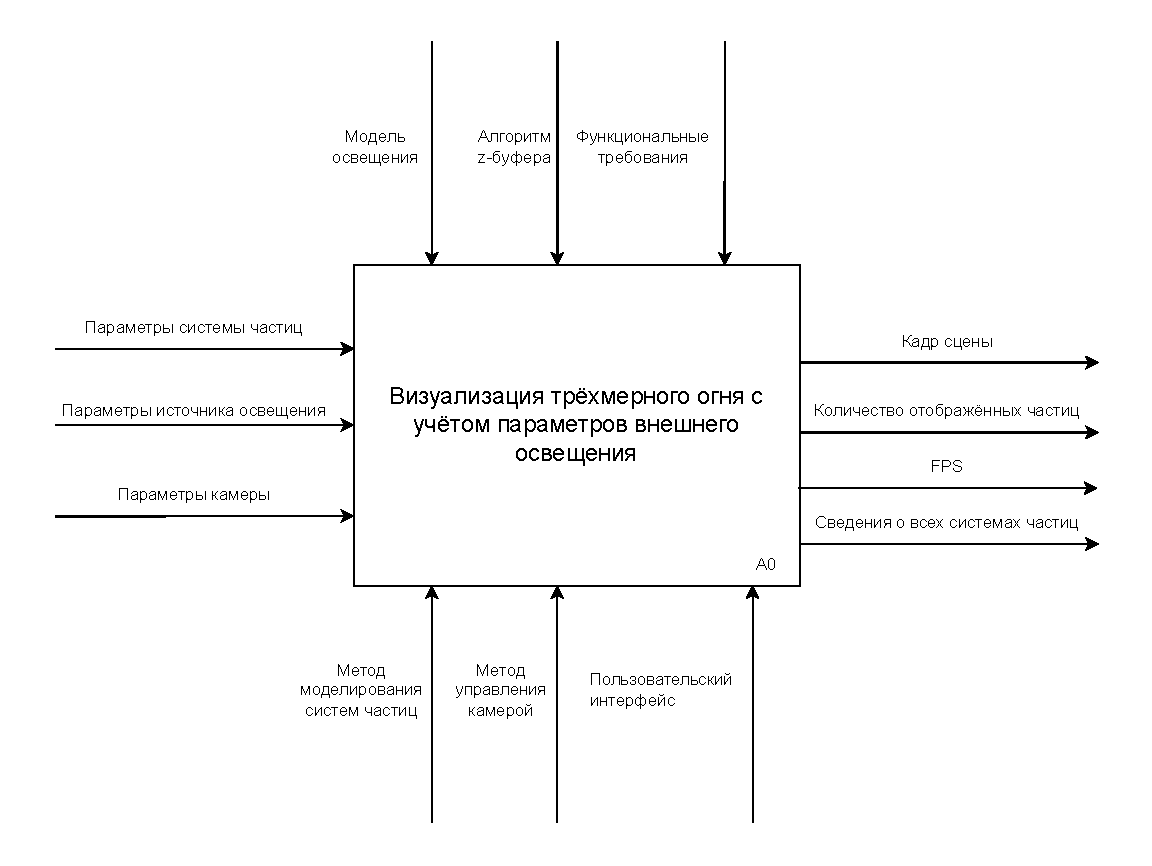
\includegraphics[width=0.99\textwidth]{idef0_main.pdf}
	\caption{Диаграмма IDEF0 нулевого уровня процесса визуализации трёхмерного огня}
	\label{fig:idef0-main}
\end{figure}

\clearpage

Полное представление основного процесса работы программы представлено в расширенной нотации IDEF0 (диаграмма первого уровня) приведено на рисунке~\ref{fig:idef0-exp}.

\begin{figure}[h!]
	\centering
	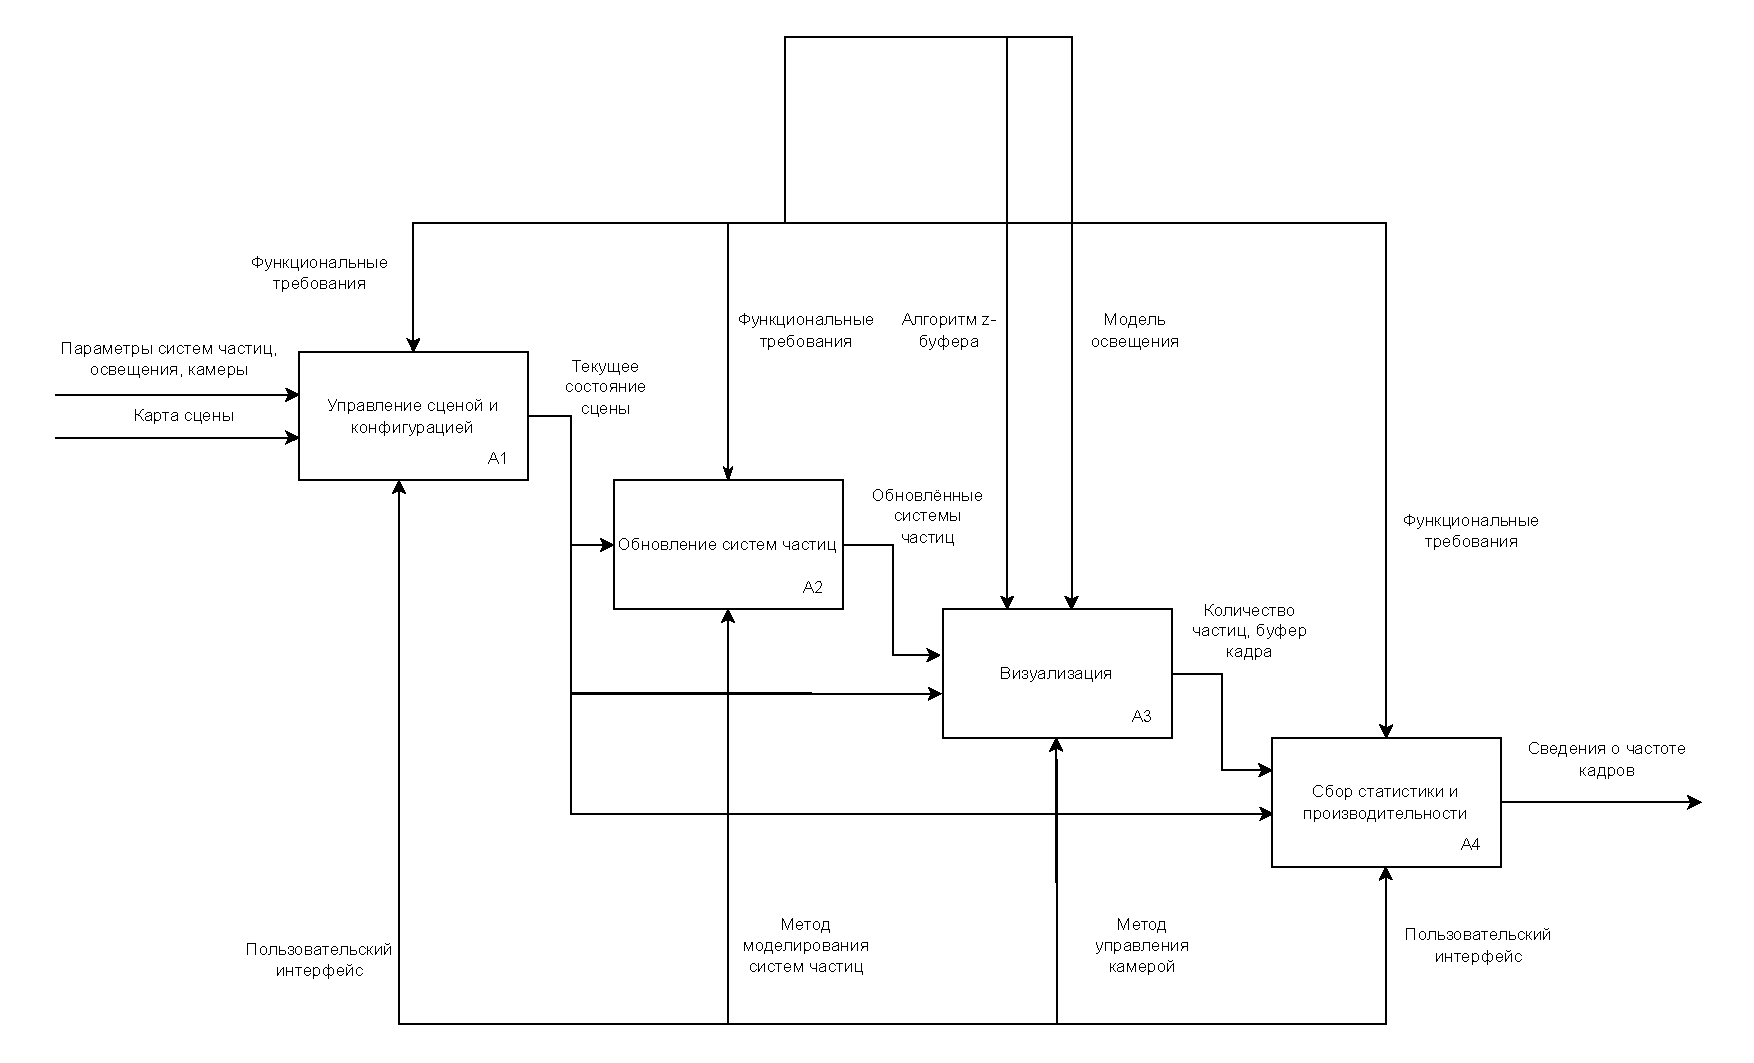
\includegraphics[width=0.99\textwidth]{idef0_expanded.pdf}
	\caption{Диаграмма IDEF0 первого уровня процесса работы программного обеспечения}
	\label{fig:idef0-exp}
\end{figure}

\clearpage

\section{Алгоритм обновления системы частиц}

Алгоритм обновления одной системы частиц реализует эволюцию частиц во времени: рождение новых частиц, изменение их положения и характеристик, удаление мёртвых частиц.

Схема алгоритма обновления системы части приведена на рисунке~\ref{fig:alg-update}.

\begin{figure}[h!]
	\centering
	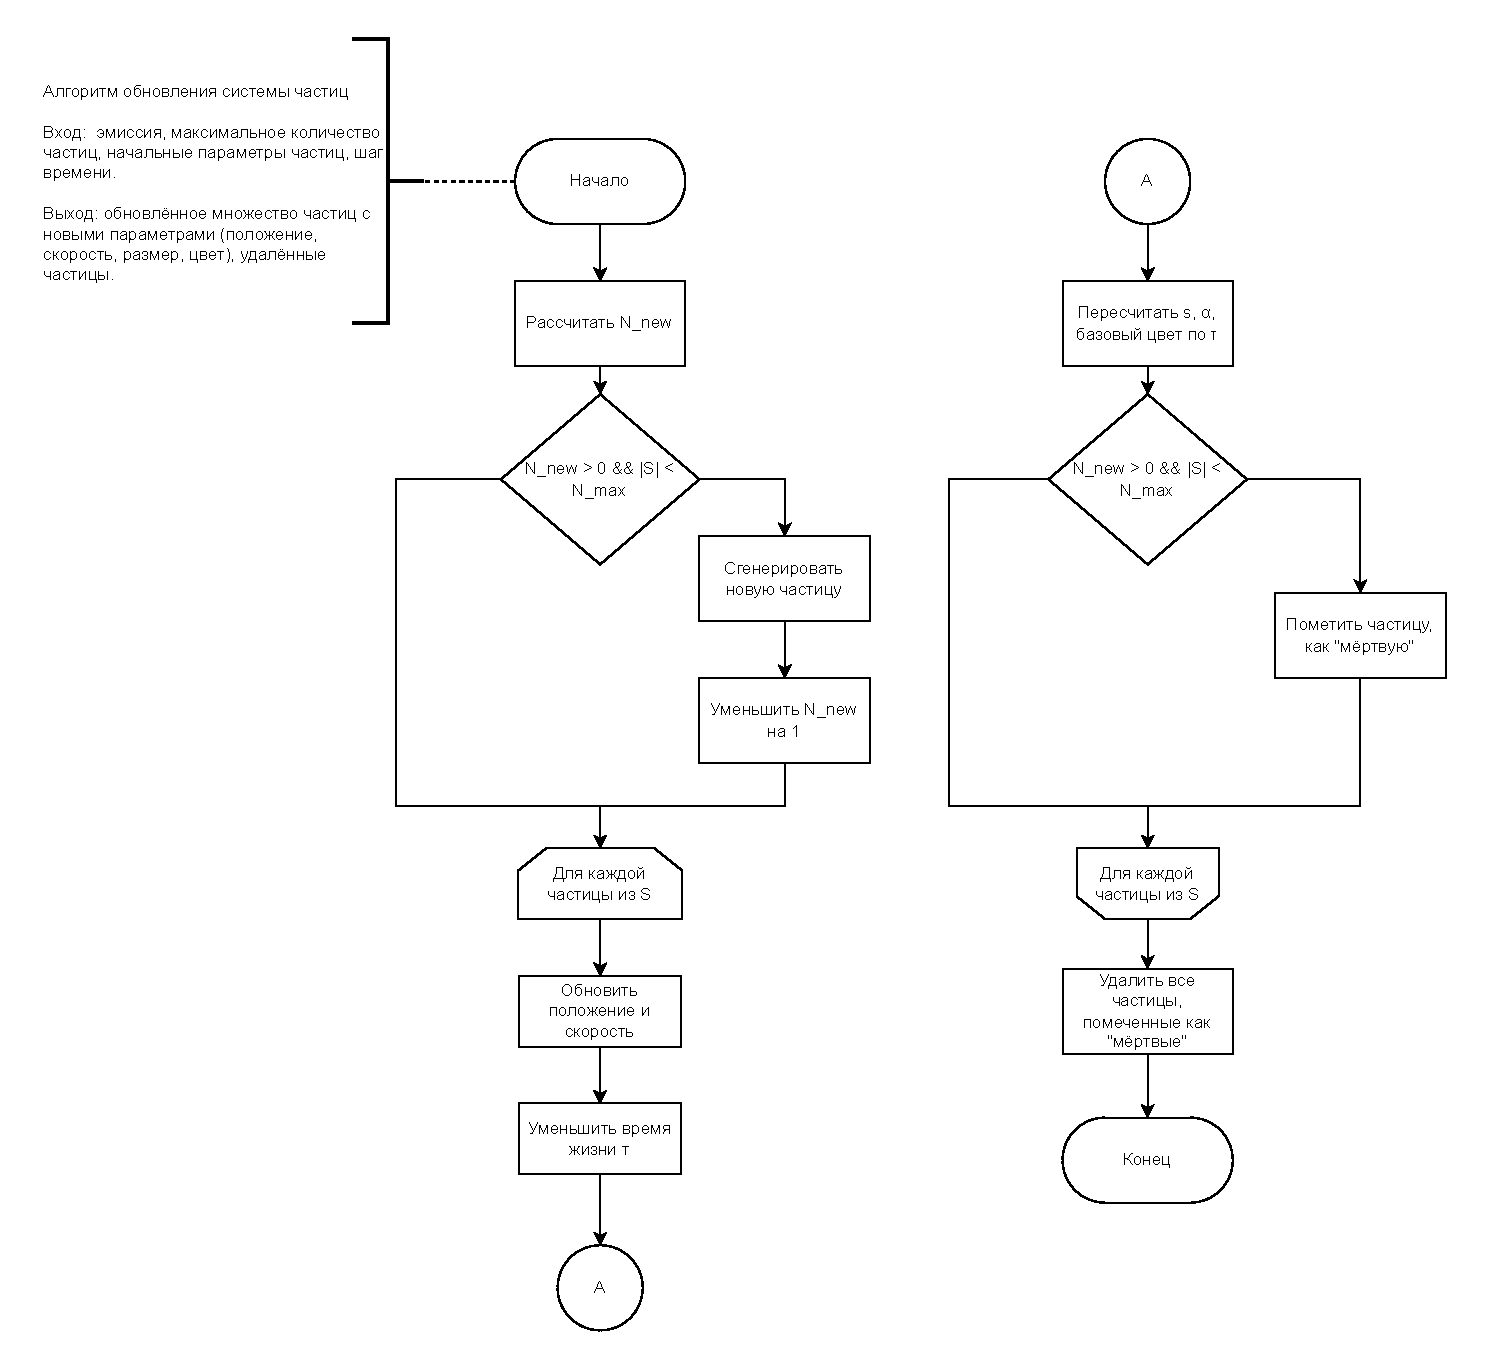
\includegraphics[width=0.99999\textwidth]{alg_update_particlesystem.pdf}
	\caption{Схема алгоритма обновления системы частиц}
	\label{fig:alg-update}
\end{figure}

\clearpage

\section{Алгоритм вычисления цвета частиц с учётом освещения}

Алгоритм вычисления цвета частиц реализует принятую в работе эмиссионную модель освещения с учётом внешнего точечного источника света.

Схема алгоритма вычисления итогового цвета частицы приведена на рисунке~\ref{fig:alg-color}.

\begin{figure}[h!]
	\centering
	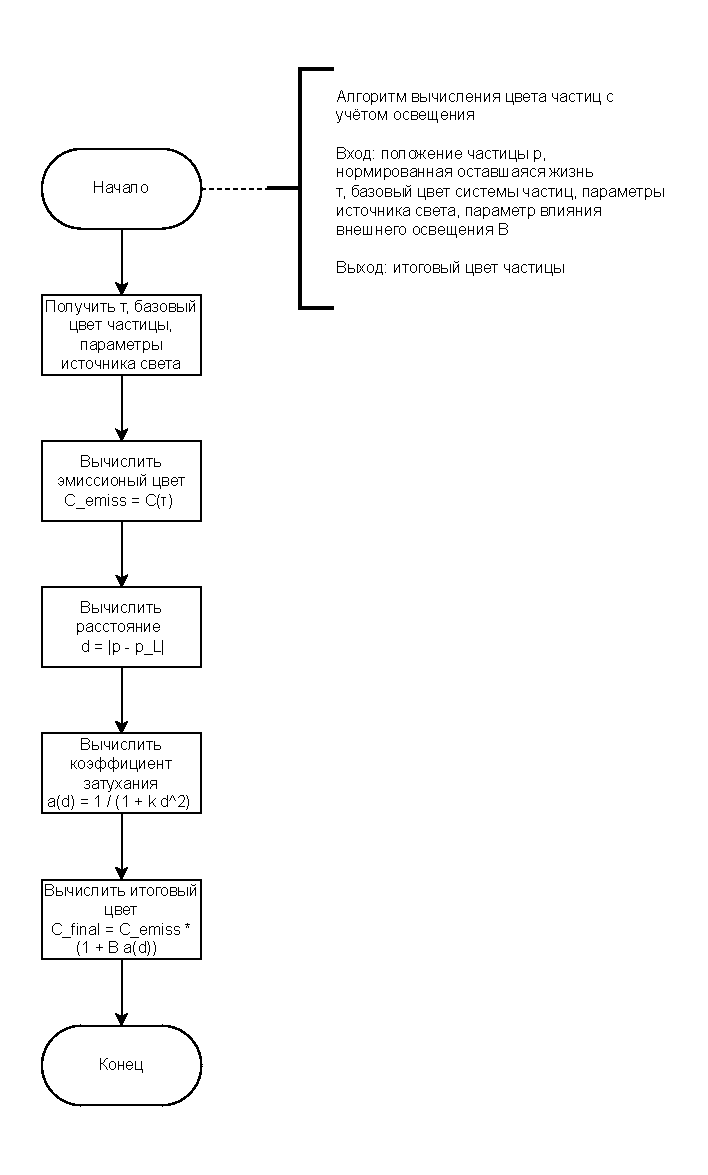
\includegraphics[width=0.7\textwidth]{alg_color_computation.pdf}
	\caption{Схема алгоритма вычисления цвета частицы с учётом освещения}
	\label{fig:alg-color}
\end{figure}

\clearpage

\section{Алгоритм визуализации сцены}

Алгоритм визуализации сцены описывает преобразование трёхмерных координат частиц в двумерное изображение с учётом перспективной проекции и удаления невидимых поверхностей.

Схема алгоритма визуализации сцены с использованием z-буфера приведена на рисунке~\ref{fig:alg-visualization}.

\begin{figure}[h!]
	\centering
	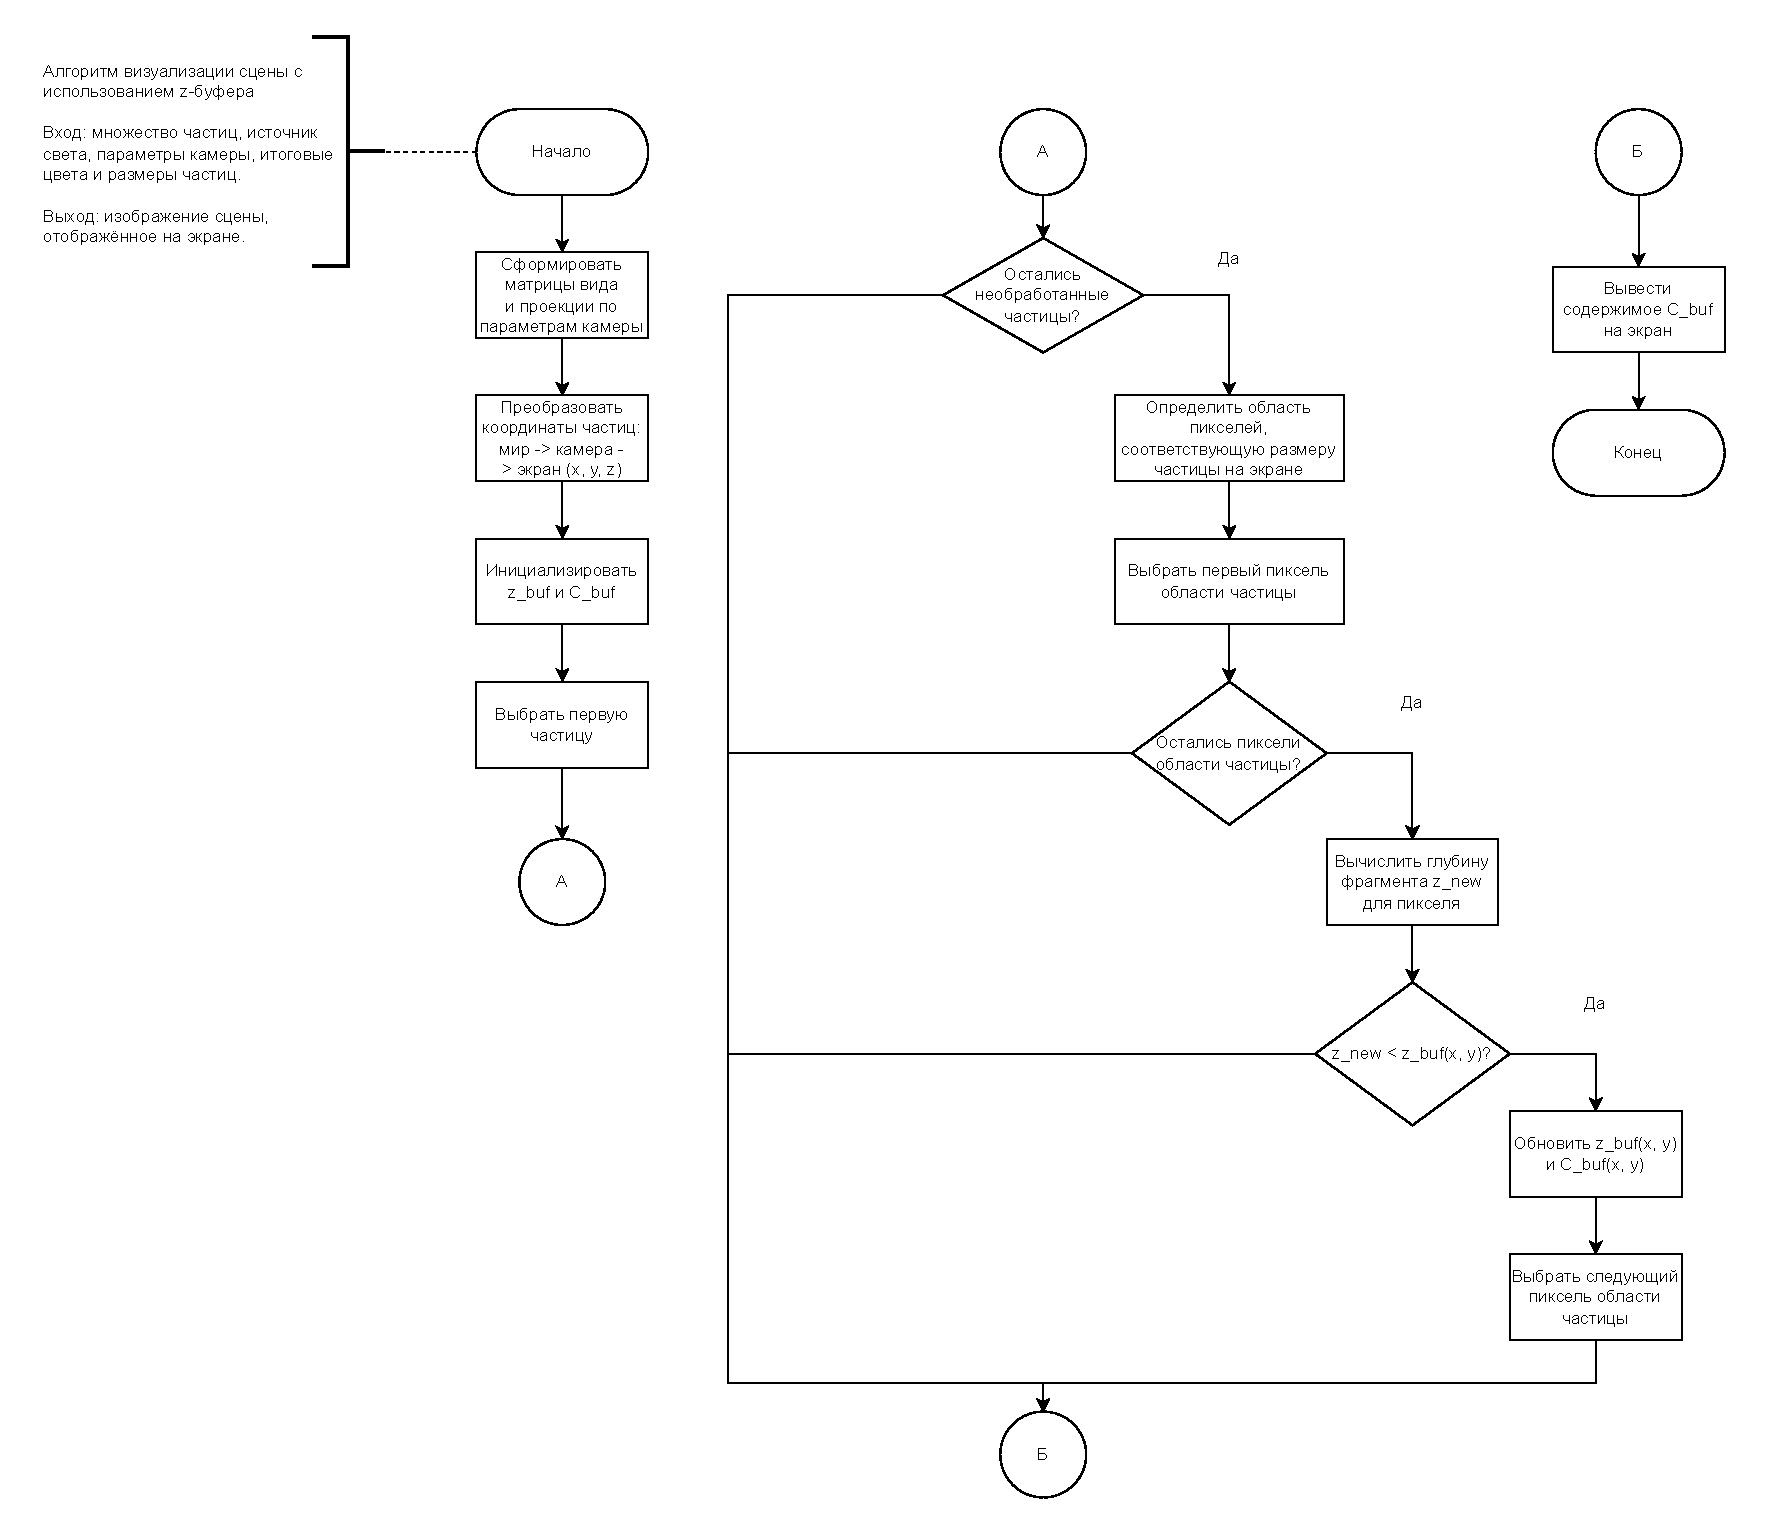
\includegraphics[width=0.9999\textwidth]{alg_visualization.pdf}
	\caption{Схема алгоритма визуализации сцены с использованием z-буфера}
	\label{fig:alg-visualization}
\end{figure}

\clearpage

\section{Вывод}

В конструкторской части сформулированы требования к программному обеспечению для визуализации трёхмерного огня методом систем частиц, разработана общая архитектура программного комплекса и формальная модель данных, описывающая основные объекты сцены.

Для ключевых алгоритмов работы программы (основной цикл, обновление систем частиц, вычисление цветов с учётом освещения, проекция и удаление невидимых поверхностей) приведены формальные описания.

\clearpage